\label{DL_theory}
\section{Deep Learning for spectroscopic data}

Techniques of machine learning and deep learning specifically have been applied to spectroscopic data since the 1990s. It has been applied to a variety of spectroscopic methods such as Near Infrared Spectroscopy (NIR), Raman Spectroscopy, Nuclear Magnetic Resonance Spectroscopy (NMR), Infrared Spectroscopy (IR) and Laser Induced Breakdown Spectroscopy (LIBS) \cite{krohling_1d_2023, sun_cnnlstm_2023, ma_conditional_2022, zhang_deep_2023, castorena_deep_2021, ghosh_deep_2019, huang_attention_2019}. However, chemometric or physics-based approaches have been and still are favored for data analysis due to the lack of model explainability for data-driven approaches. Because chemometrics is most often based on decomposition techniques such as Principal Component Analysis (PCA) and subsequent linear regression, it remains possible to interpret why a model predicts something by considering the loadings (weights) of the selected (principal) components. However, especially because of the non-linear learning capabilities of deep learning, they have been widely applied chemical analysis methods with complex underlying physical effects \cite{aires-de-sousa_prediction_2002}.

Deep learning has been previously applied to XPS-analysis by Drera et al.\cite{drera_deep_2019}. They achieved an overall performance of quantitative detection above 10$\%$ content, similar to the detection limit of users - they state. They used solely convolutional neural networks to build their prediction model. Their training data was constructed similarly to the data used in this work. Moreover, Hunt investigated depth profiling using XPS in combination with the singular value decomposition (SVD) algorithm \cite{hunt_depth_2000}. Additionally, Hunter modelled the impact of sample surface roughness on the prediction using the SVD algorithm and the Tyler regularization algorithm.

Attention-based neural networks have been applied to near infrared spectroscopy analysis of medical fungi \cite{huang_attention_2019} and sand gravel \cite{yuan_hybrid_2022} to successfully identify secondary parameters, such as moisture or polysaccharide content with similar or better results than the well-known partial least squares (PLS) fitting.

% advances in DL & applications to spectroscopy tasks

\subsection{Model hyperparameters \& training}
For each model, a set of hyperparameters define either initial, or fixed values used for the training. 

Multiple training cycles are performed on the dataset, which is shuffled before each training cycle, also called epoch. A so-called \emph{loss function} is introduced which in general resembles how far the predicted $\hat{y}$ labels are from the correct labels $y$ $(\hat{y} - y)$.
In each epoch, the weights of the model are re-evaluated subject to minimizing the defined loss-function. This re-evaluation is done with gradient-based methods, before the weights are changed based on the computed gradient multiplied with the defined learning rate. The initial data available is split into a training and validation dataset. The weights are trained only on the training dataset, while the validation dataset is used to check the performance on data which is new for the model and tune its hyperparameters. Model training is successful if we observe the training data loss decrease over the epochs. 


\subsection{General patterns}
\subsubsection{Loss functions and performance measures}
 A loss function generally computes how close the model predictions are to the labels, while the accuracy will describe what proportion of labels were predicted correctly. As the task can be of several types, such as regression, or classification, the loss and accuracy functions should be adapted accordingly. The functions used in this work will be explained hereafter.
The categorical crossentropy loss function is used for multi-class and multi-label classification problems. It is computed according to equation \ref{cce}, where $M$ is the number of classes, $y$ is the ground-truth and $p$ is the prediction of the observation $o$ of class $c$ \cite{noauthor_classical_nodate}. 
Categorical Accuracy computes the correctly predicted label based on the argmax function (the highest prediction value) of one-hot encoded labels.
\begin{equation}
\label{cce}
-\sum_{c=1}^My_{o,c}\log_{n}(p_{o,c})
\end{equation}

\begin{equation}
\label{cce}
\text{Categorical Cross-Entropy} = -\sum_{c=1}^My_{o,c}\log_{n}(p_{o,c})
\end{equation}
For problems where the labels are non-exclusive (multiple can be true) the mean absolute error loss can be used. This is based on the equation \ref{eq:MAE}.
 \begin{equation}
 \label{eq:MAE}
     \text{Mean Absolute Error} = \frac{1}{n}\sum_{i=1}^{n} |y_i - \hat{y}_i|
 \end{equation}
 
\subsubsection{Dense layers}
What is often referred to as fully connected, dense, feed-forward neural network or Multilayer Perceptron describes a network consisting of solely fully connected layers. These layers are connected in an $n:m$ manner, where each node of a layer with $n$ nodes is connected with each node of another layer with $m$ nodes. 

\subsubsection{Dropout}
Dropout layers are often used to regularize and generalize models. In these layers, which are fully connected layers, a certain percentage of nodes are not used during training and the specific unused nodes are selected from new each training cycle. This ensures that the training of the network does not rely on only a subset or even a single node, but on all nodes in a similar intensity. The fraction of nodes defined to drop each training cycle is denoted as $p$.

\subsubsection{Batch-Normalization}
Big datasets are usually divided into subsets such that we can efficiently train our network. This is done because the data might not fit the available computing memory and thus slow our computation. However, even if we randomly split the dataset, we will encounter a non-uniform distribution of information between our batches. Thus, in a batch-normalization layer, each batch input is normalized to have a mean of zero and a standard deviation of one. 
%The positive effects have been shown in multiple publications

\subsection{Convolutional Neural Networks (CNN)}
In convolutional neural networks (CNN), the input values are multiplied with a kernel to extract features. The CNNs are used where the input is of a discrete, grid-like topology. A kernel in this sense can represent a vector of n dimensions, where in case of spectra n=1, that will be moved along an axis (x-axis in for spectra), applying the multiplication subsequently. As the kernel can not be applied at the ends of our data, we can decide to apply padding on the ends with zero values, or start only when the kernel fits our data. Applying a kernel of size 5 on a vector of length 20 will thus only compute a vector of size 11 without padding, whereas its length will be 20 with the padding.
The values of the kernel are learnable, such that it can be fitted to extract specific features depending on the nature of the data.

These convolutional layers are usually followed by pooling layers - such as max-pooling or average-pooling - which also use a kernel. As the pooling layers reduce the dimensionality of the input, they have a number of positive effects on the model, such as better robustness to input variability and faster training. In addition, pooling layers help the model to learn invariances in the input data, such as rotation or small shift of an image content \cite{goodfellow_deep_2016}. 

The 1-dimensional convolutions we use in the case of spectral data will thus use $p$ one-dimensional kernels (vectors) of pre-defined length, where $p$ stands for the number of channels. If, for example, our spectrum vector is of length 1024, using a 1d-convolutional kernel of arbritary size with 16 channels will be applied. Thus, we will retain 16 vectors, each representing a convoluted feature of our spectrum. Arranging multiple CNN layers in sequence is a usual architecture used, as the layers learn from previously extracted features to represent more complex structures.

This network architectural pattern is extensively used in image classification tasks but has also been applied to diverse classification tasks, including spectroscopic data analysis \cite{sun_cnnlstm_2023, castorena_deep_2021, drera_deep_2019}.

\subsection{Residual networks (ResNet)}

In residual networks, the input is re-added after performing weighted operations such as convolutions. This feature has known positive effects, especially on deeper neural networks (networks with multiple layers). Residual network architectures diminish the well-known vanishing gradient problem by adding skip connections to the network. 

\begin{figure}[H]
    \centering
    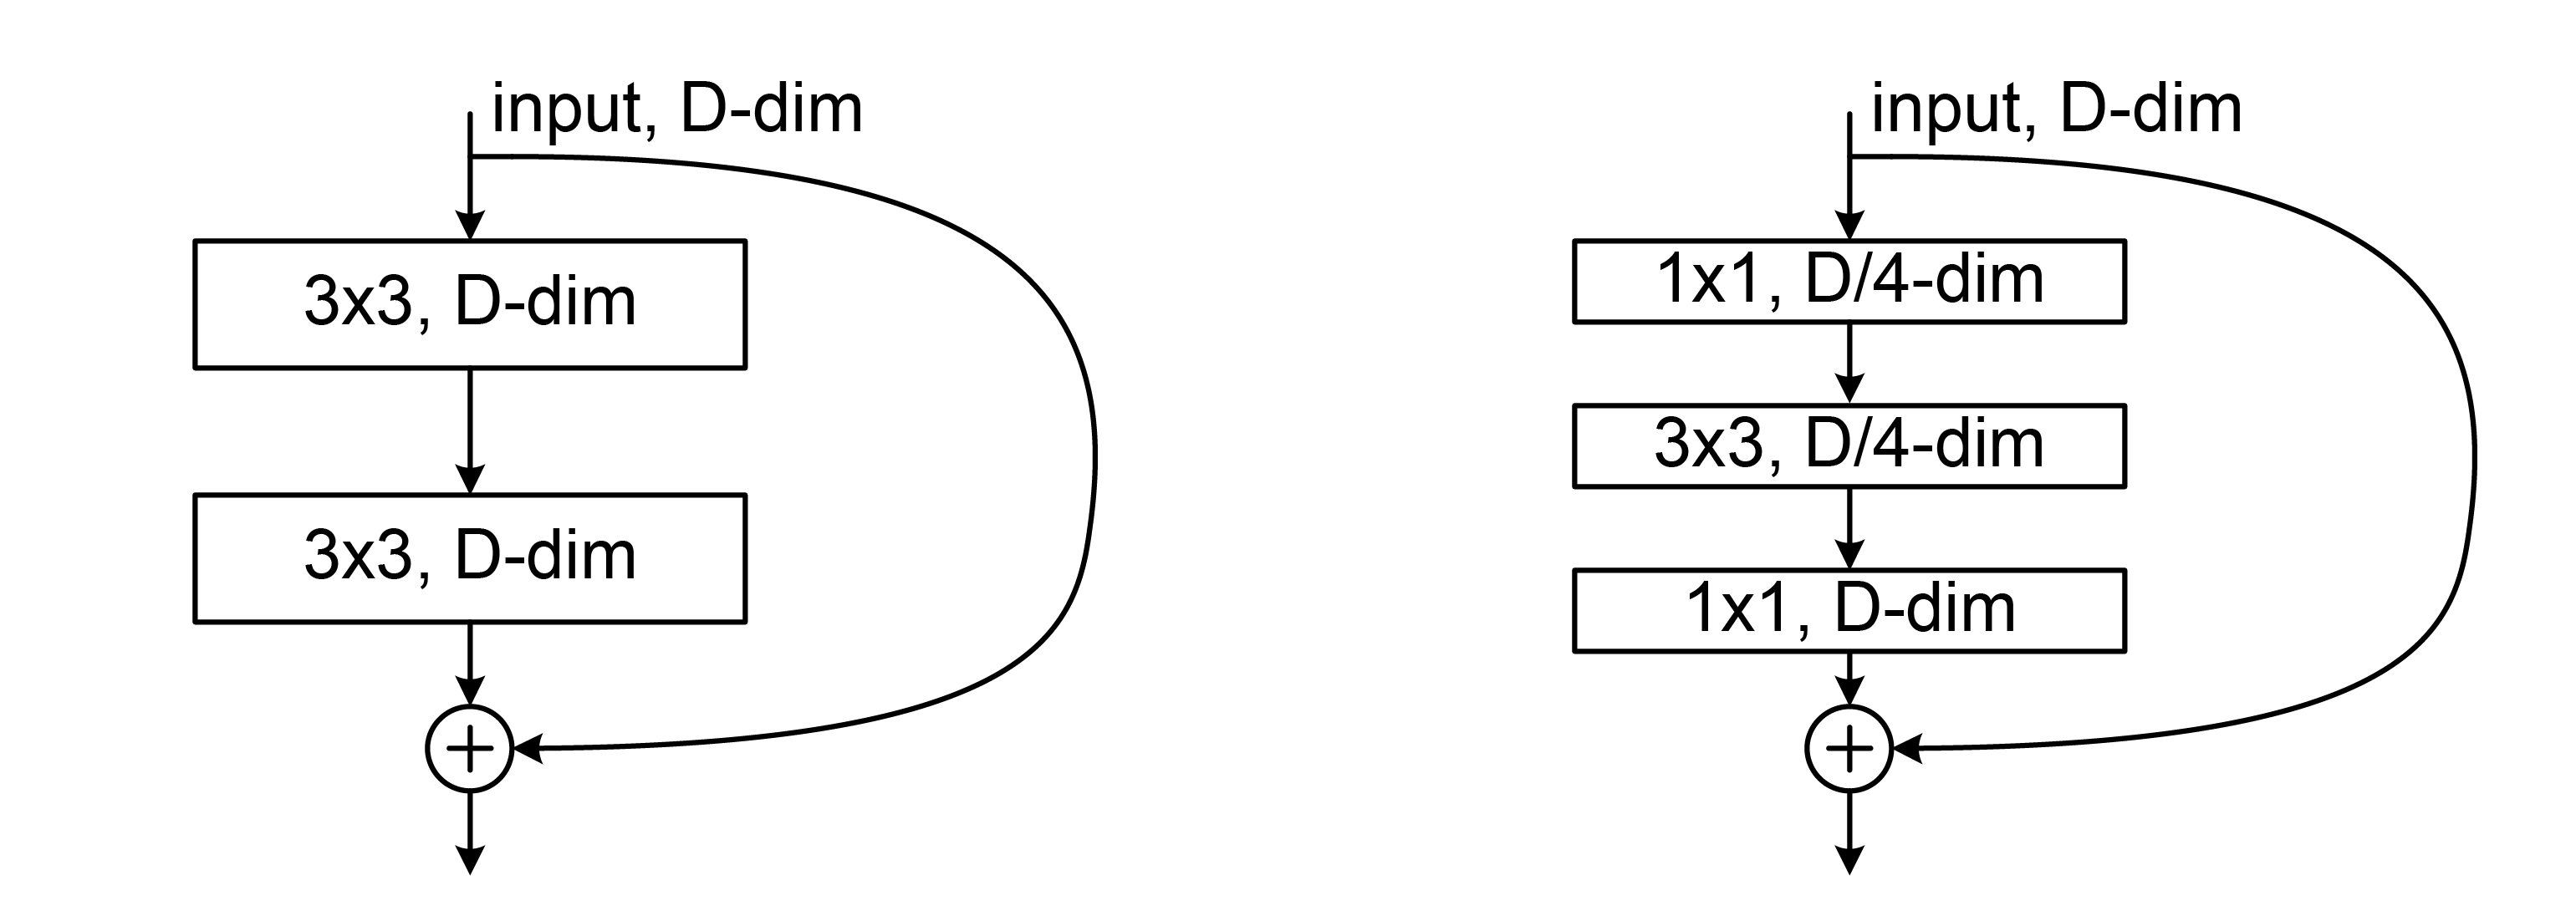
\includegraphics[width=0.5\textwidth]{Figures/ResBlockVariants.png}
    \caption{Residual block pattern}
    \label{fig:res_block}
\end{figure}

This pattern has later also been used for other models, as it allows much deeper networks to learn much more efficiently. Especially, in combination with convolutional models, this has improved the accuracy eg. in CBAM as explained below.

\subsection{Transformer-based networks}

Originally developed to solve neural language processing (NLP) tasks, the attention mechanism was first described in 2017 \cite{vaswani_attention_2023}.
The combination of an encoder-decoder paradigm with the Multi-Head Attention architecture lead to the development of the Transformer model. The most recent architecture used for NLP tasks is shown in Figure \ref{fig:transformer_model}.
A transformer consists of tokenizers, embedding layers and transformer layers which include the attention layers and multilayer perceptron (MLP) layers.

\begin{figure}[H]
    \centering
    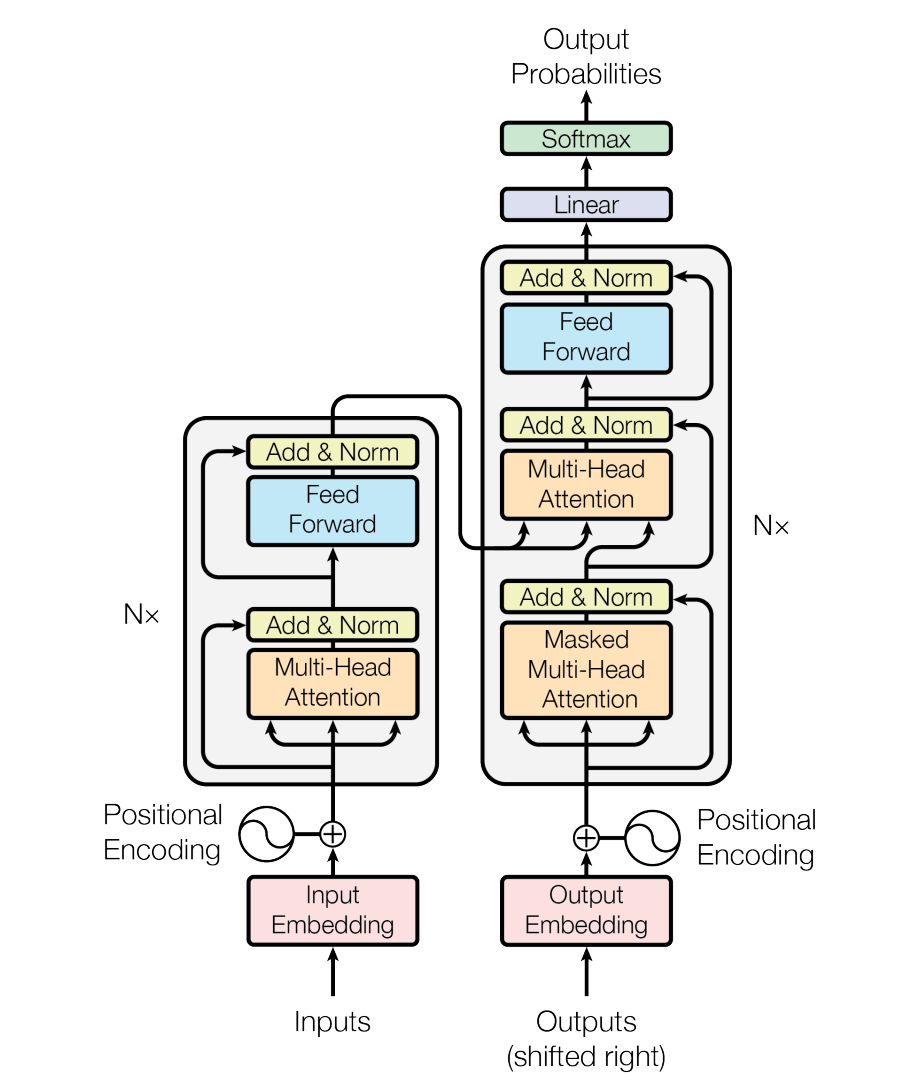
\includegraphics[width=0.6\textwidth]{Figures/Transformer.png}
    \caption{The Transformer-model architecture \cite{vaswani_attention_2023}}
    \label{fig:transformer_model}
\end{figure}

The positional embedding ensures that the model can interpret the position of the tokens within the sequence. The Multi-Head Attention block consist of linear input mappings to query, key and value pairs which are run in parallel. With the query and key mappings, an attention matrix is computed which is concatenated with our value matrix after applying softmax-normalization.  \cite{vaswani_attention_2023}. 

\subsubsection{Convolutional Block Attention Module (CBAM)}
The Convolutional Block Attention Module (CBAM) connects the attention paradigm with the convolutional approach and consists of two sub-modules. Inputs are convoluted, and with the first module, a 1D channel attention map on the convolution-channels is generated. Afterwards, these channel attentions are used as an input to the spatial attention module to compute the spatial attention. This means that the model is then able to learn which channels and which regions of the input data are more important than others. These two blocks can then be integrated within a convolutional based network or a residual based network.

\begin{figure}[H]
    \centering
    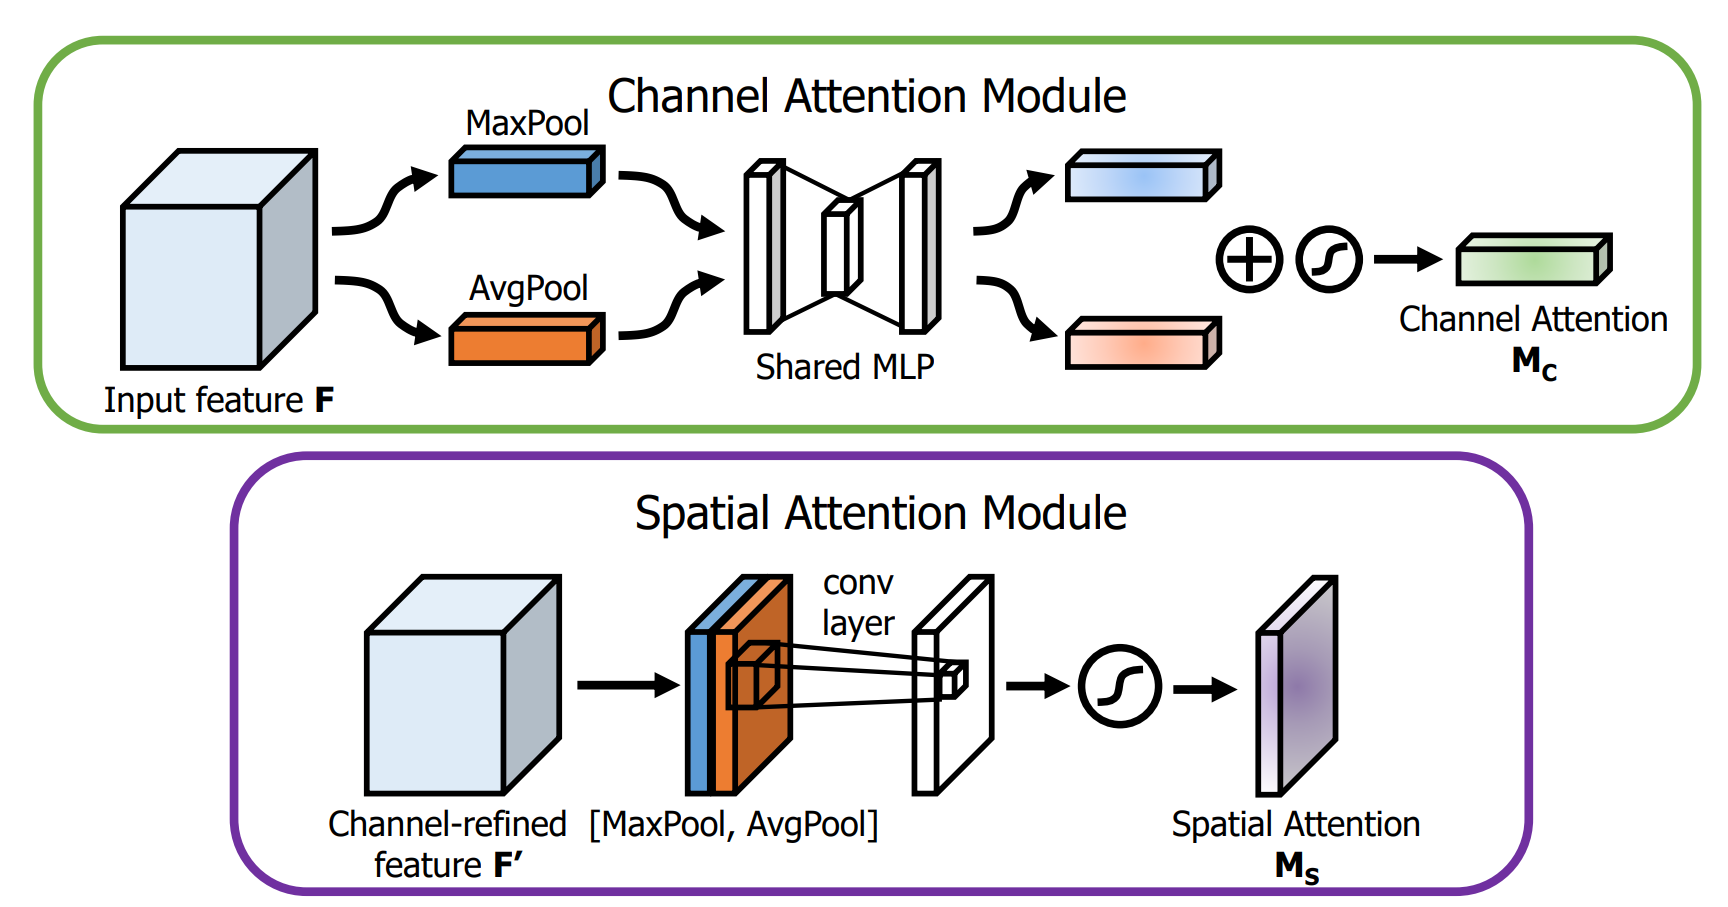
\includegraphics[width=0.8\textwidth]{Figures/cbam_modules.png}
    \caption{Channel \& Spatial attention module blocks \cite{woo_cbam_2018}}
    \label{fig:cbam_modules}
\end{figure}

\begin{figure}[H]
    \centering
    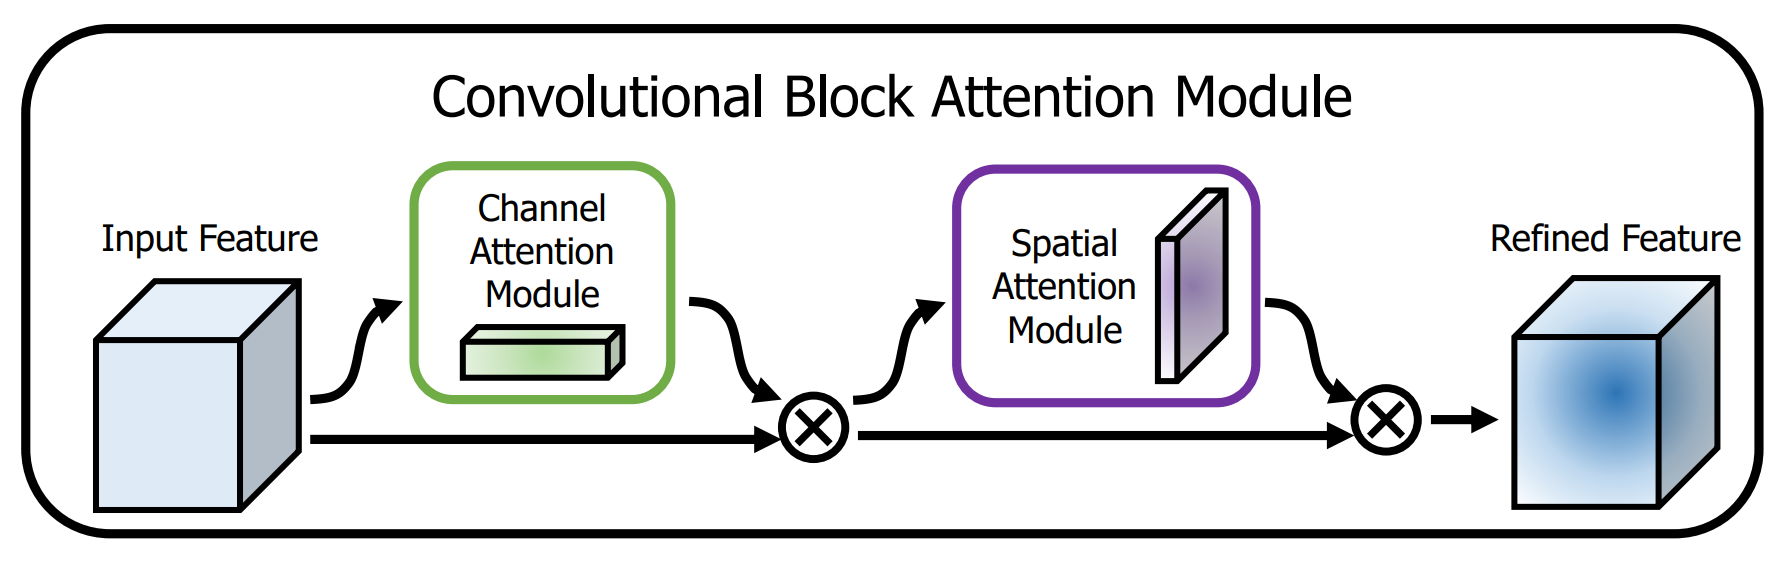
\includegraphics[width=0.7\textwidth]{Figures/cbam_modul.png}
    \caption{CBAM-architecture \cite{woo_cbam_2018}}
    \label{fig:cbam}
\end{figure}


\begin{figure}[H]
    \centering
    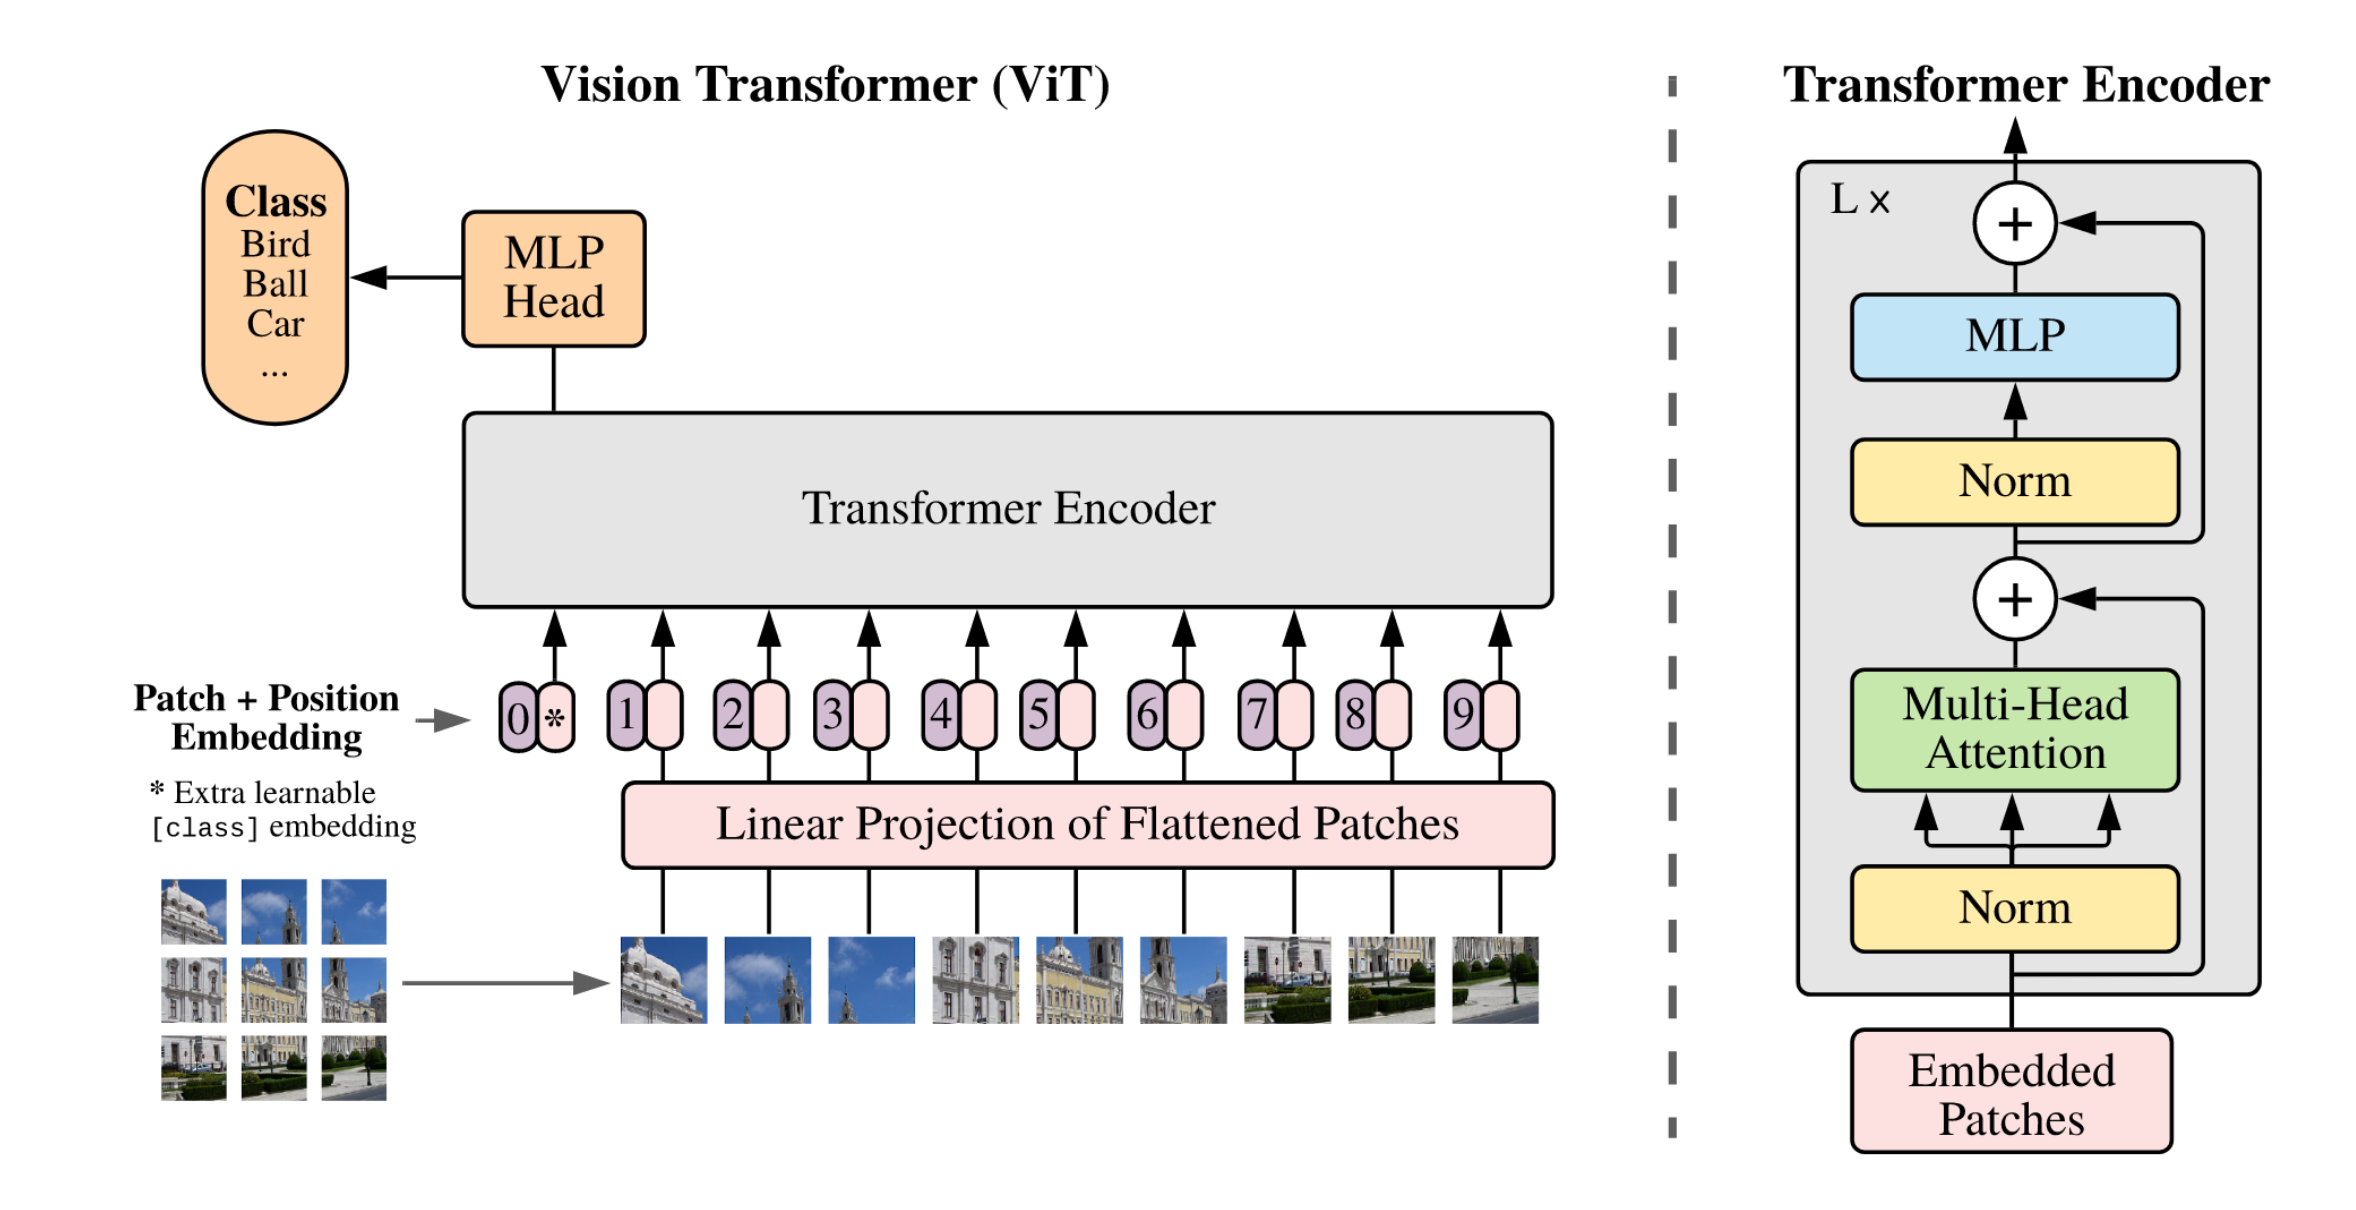
\includegraphics[width=0.8\textwidth]{Figures/ViT.png}
    \caption{Vision Transformer \cite{dosovitskiy_image_2021}}
    \label{fig:vit_model}
\end{figure}

\subsubsection{Vision Transformer (ViT)}
The Vision transformer model (ViT) has been recently published \cite{dosovitskiy_image_2021} and uses the mechanisms of Transformer-based models for computer vision tasks. As shown in Figure \ref{fig:vit_model}, it only uses the encoder part of the transformer. The input data is divided into multiple patches of size n, similarly to tokenized words in natural language processing. A positional embedding is computed - this encodes the position in a unique way. The embedded patches are then used as tokenized input to the transformer encoder. In the encoder, the patches are fed through $L$ subsequent Multi-Head Attention blocks. Lastly, the last encoder block outputs are fed into a MLP-Head which itself is connected to the output-layer representing the classes to be predicted.
